% --------------------------------------------------------------
% This is all preamble stuff that you don't have to worry about.
% Head down to where it says "Start here"
% --------------------------------------------------------------
 
\documentclass[a4paper, 12pt]{article}
 
\renewcommand{\baselinestretch}{1.0}
\usepackage[margin=1in]{geometry} 
\usepackage{amsmath,amsthm,amssymb}
\usepackage{blindtext}
\usepackage{german}
\usepackage{hyperref}

\usepackage{graphicx}
\graphicspath{ {./images/} }

\begin{document}
 
% --------------------------------------------------------------
%                         Start here
% --------------------------------------------------------------
 
%\renewcommand{\qedsymbol}{\filledbox}
 
\title{Project Bloom}
\author{Carlo Baumann, Peer J\"uttner\\
Bonusaufgabe - Bloomfilter}
 
\maketitle

\section{JAVA-Programm} 
Zur Erstellen war ein JAVA-Programm, das folgendes leistet:\newline
Bei einer gegebenen Anzahl \textit{n} an zu erwartenden Elementen, die in der Datenstruktur gespeichert werden und einer Fehlerwahrscheinlichkeit p wird eine geeignete Filtergr\"osse \textit{m} und die optimale Anzahl \textit{k} an Hashfunktionen berechnet.
Das JAVA-Programm kann unter folgendem Link heruntergeladen werden:
\url{https://github.com/peerjuettner/project-bloom.git}
\section{Idee Bloom Filter} 
\subsection{Vor- und Nachteile}
Ein grosser Vorteil des Bloom Filter ist die effiziente Nutzung und der kleine Speicherbedarf. Dies macht ihn \"ausserts platzsparend und effizient. Er muss im Gegensatz zu Sets nicht die komplette Datenstruktur abbilden, sondern nur die Hash-Werte.

Der Bloom Filter sagt aber nicht aus, ob ein Element vorhanden ist. Er kann lediglich aussagen, ob ein Element nicht vorhanden ist. Wenn der Bloom Filter einen Treffer zur\"uckgibt, er also meint er habe das Element gefunden. Besteht immernoch eine Wahrscheinlichkeit von 1\%, dass das Element nicht vorhanden ist.


\subsection{Praxisbeispiel}
Der Algorithmus, f\"ur eine gute Verteilung des Hashes, findet unter anderem in den Programmiersprachen, beispielsweise Java, oder auch in den Relationalen Datenbanken Anwendung.

Ein weiterers Beispiel ist die Anwedung bei Bitcoins. Bitcoin ist eine sogenannte Kryptow\"ahrung. Bitcoin ist eine Geldeinheit aber auch ein Zahlungssystem. Das System basiert auf einer von allen Teilnehmern verwalteten Datenbank, der Blockchain. In der Blockchain werden alle Transaktionen aufgezeichnet, welche jemals durchgef\"uhrt wurden. Diese Blockchain wurde \"uber die Jahre immer gr\"osser. Um es nun auch mobilen Klienten zu erm\"oglichen am System teilzunehmen, wurde das SPV (Simple Payment Verification) Verfahren entwickelt. Dieses basiert auf dem Bloom Filter. Das SPV dient dazu nur die f\"ur den Klienten relevanten Transaktionen herauszufiltern. Mit dem Bloom Filter wird getestet, ob die Transaktion bereits in der Blockchain vorhanden ist. Dazu wird ein Membership Test gemacht. Dieser pr\"uft, ob der Hash der Transaktion bereits in der Blockchain vorhanden ist.
\medskip
\par
\begin{center}
{%
\setlength{\fboxsep}{1pt}%
\setlength{\fboxrule}{1pt}%
\fbox{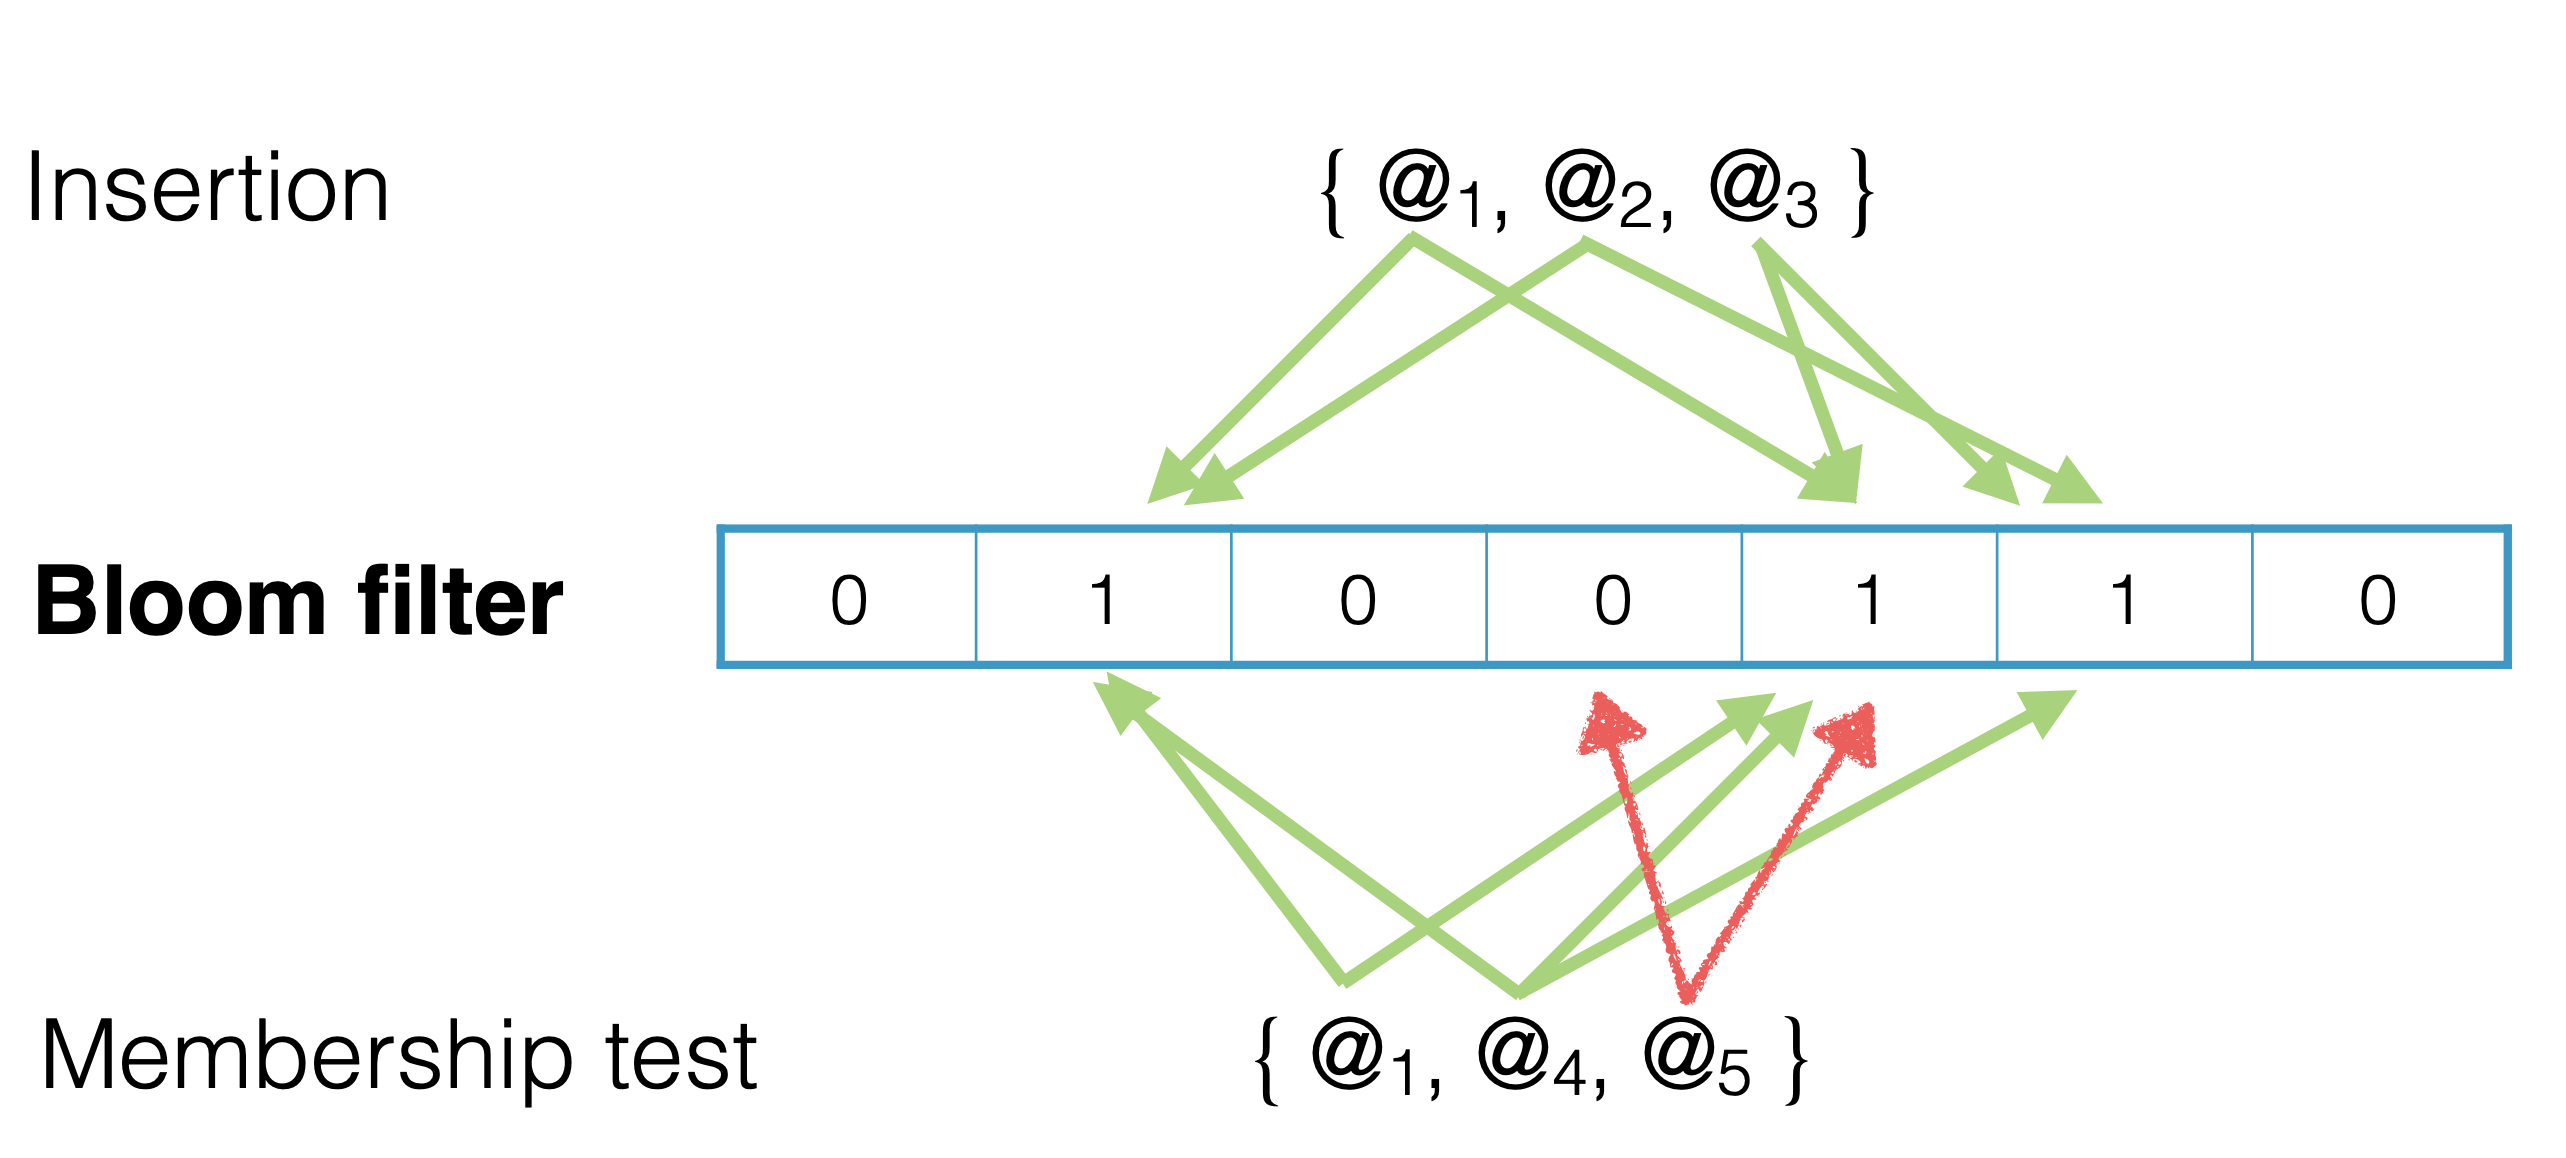
\includegraphics[scale=0.3]{images/spv.png}}%
}%
\newline \textit{Membership Test}
\footnote{\url{https://www.ethz.ch/content/dam/ethz/special-interest/infk/inst-infsec/system-security-group-dam/research/publications/pub2014/acsac_gervais_slides.pdf}}
\end{center}
\medskip
\par
Mit Hilfe des SPV und dem Bloom Filter, konnte die Leistung des Bitcoin Netzwerks erh\"oht werden, da nicht mehr die komplette Blockchain abgeglichen werden muss.


\subsection{Tests}
Wir haben das Programm durch \"andern der Werte von \textit{p} getestet. Bei einer Wahrscheinlichkeit von 1.0 hat sich gezeigt, dass wir nur False-Positive Treffer haben. Dies war so zu erwarten. Variiert man\textit{p} im Prozent-Bereich so sieht man, dass im Mittel der erwartetet Wert dem effektiven Wert entspricht.

\begin{center}
\begin{tabular}{ |c|c|c|c| } 
 \hline
 Anzahl Test-W\"orter & 10'000 & 10'000 & 10'000 \\
 k & 6 & 5 & 0 \\ 
 m & 556987 & 473152 & 0 \\ 
 n & 58110 & 58110 & 58110 \\
 p erwartet & 0.01 & 0.02 & 1.0 \\ 
 p & 0.0107 & 0.0214 & 1.0 \\ 
 False-Positiv Treffer & 100 & 214 & 10000 \\ 
 \hline
\end{tabular}
\end{center}


\begin{thebibliography}{9}
\bibitem{paper} 
Gervais, Arthur and Capkun, Srdjan and Karame, Ghassan O. and Gruber, Damian
\textit{On the Privacy Provisions of Bloom Filters in Lightweight Bitcoin Clients}. 
Proceedings of the 30th Annual Computer Security Applications Conference, New Orleans, Louisiana, USA, 2014.

\end{thebibliography}
 
\end{document}